% Szymon
\section{Kolorowania węzłów}
W niniejszej części zostanie przedstawione zagadnienie kolorowania węzłów. Podana zostanie definicja kolorowania, oraz warunki które muszą zostać spełnione aby węzeł mógł zostać w określony sposób pokolorowany. Następnie zdefiniowane zostaną równania kolorowań oraz macierze kolorowań. Ostatnim etapem będzie wprowadzenie macierzy kolorowań jako niezmiennika węzłów. 

\subsection{Kolorowanie diagramów}

Niech K będzie węzłem zorientowanym, L jego diagramem, A zbiorem łuków,  C = $\lbrace c_{1}, \ldots, c_{k}\rbrace$ zbiorem skrzyżowań. 

\begin{definicja}
Diagram L jest kolorowalny modulo $n \in \N$, gdy każdemu łukowi diagramu L można przyporządkować liczbę $a_{i} \in \lbrace 0, \ldots, n-1 \rbrace$ taką że: \\ \\
	\begin{minipage}{0.7\textwidth}
	
	\begin{enumerate}
		\item Dla każdego skrzyżowania $c_{j}$ spełnione jest równanie kolorowania \\ $a_{m2}+a_{m3}-2a_{m1} \equiv 0$ mod n
		\item Kolorowanie nie jest stale, tzn istnieją łuki $a_{m1}, a_{mj}$ którym 			przyporządkowano różne liczby.
		 
	\end{enumerate}
	\end{minipage}
	\begin{minipage}{0.3\textwidth}
	\begin{center}

	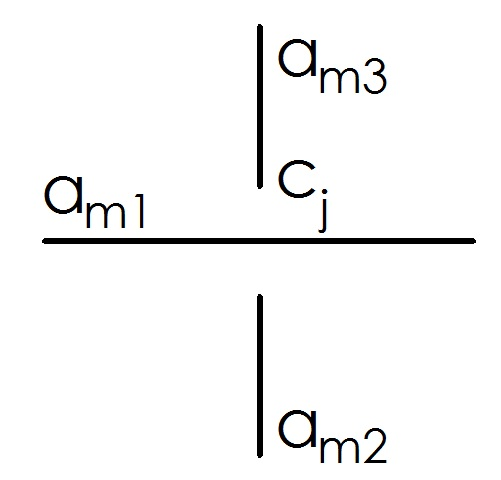
\includegraphics[scale=0.2]{2/Obrazy/Crossing1}
	\end{center}
	\end{minipage}
\end{definicja}
Przyporządkowanie spełniające powyższe własności nazywa się \emph{kolorowaniem diagramu mod n}.




\begin{twierdzenie} Kolorowalność modulo n jest niezmiennikiem węzła.
\end{twierdzenie}
\begin{proof}
Dwa węzły $L_{1}, L_{2}$ są równoważne jeżeli istnieje ciąg ruchów Reidemeistera przekształcający $L_{1}$ w $L_{2}$. Wystarczy zatem sprawdzić że kolorowalność modulo n nie zmienia się po wpływem ruchów Reidemeistera.

\begin{enumerate} \item Pierwszy ruch Reidemeistera: 

	\begin{minipage}{0.5\textwidth}
	Dla skrzyżowania $c_{j}$ spełnione jest równanie \\ $a_{m1}+a_{m2}-2a_{m2} \equiv 0$ mod n. Zatem $a_{m1} \equiv a_{m2}$.
	\end{minipage}
	\begin{minipage}{0.5\textwidth}
		\begin{center}
			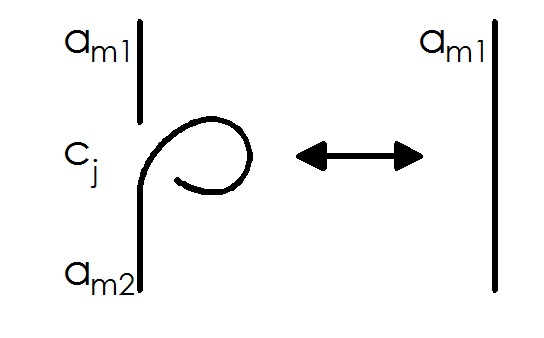
\includegraphics[scale=0.3]{2/Obrazy/R1}
		\end{center}
	\end{minipage}
\item Drugi ruch Reidemeistera: 

	\begin{minipage}{0.5\textwidth}
	Dla skrzyżowania $c_{j1}$ mamy $a_{m1}+a_{m4}-2a_{m2} \equiv 0$ mod n. Dla skrzyżowania $c_{j2}$, $a_{m3}+a_{m4}-2a_{m2} \equiv 0$ mod n. Stąd $a_{m1} \equiv a_{m3} $ mod n.
	\end{minipage}
	\begin{minipage}{0.5\textwidth}
		\begin{center}
			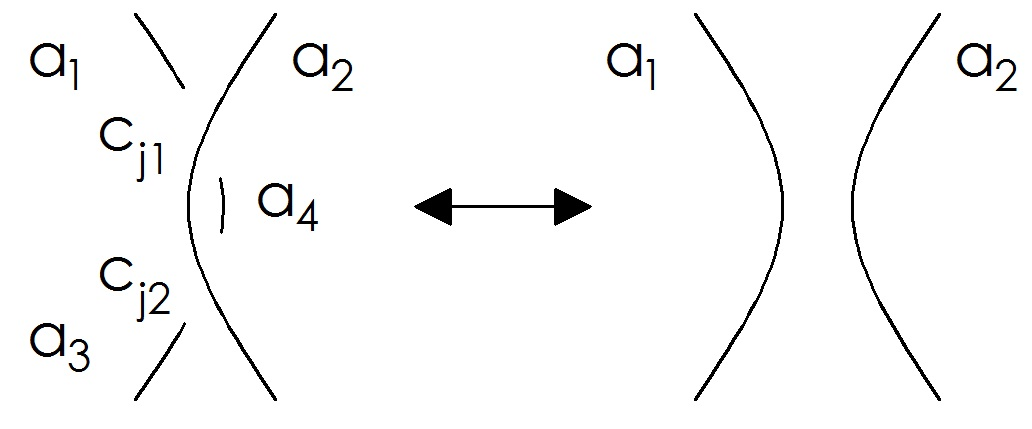
\includegraphics[scale=0.3]{2/Obrazy/R2}
		\end{center}
	\end{minipage}
	
\item Trzeci ruch Reidemeistera: 


	Dla skrzyżowania $c_{j2}$ mamy $a_{m5}+a_{m2}-2a_{m3} \equiv 0$ mod n. Analogicznie dla skrzyżowania $c_{j5}$, $a_{m8}+a_{m2}-2a_{m3} \equiv 0$ mod n. Stąd $a_{m8} \equiv a_{m5}$ mod n. \\
	\begin{minipage}{0.35\textwidth}
	W drugim przypadku mamy:\\
	$a_{m4} \equiv 2a_{m2}-a_{m1}$. \\
	$a_{m6} \equiv 2a_{m3}-a_{m4} \equiv$ \\$\equiv 2a_{m3}-2a_{m2}+a_{m1} $.	\\
	$a_{m8} \equiv 2a_{m3}-a_{m2}$. \\	
	$a_{m7} \equiv 2a_{m3}-a_{m1}$.\\		
	$a_{m9} \equiv 2a_{m8}-a_{m7} \equiv$ \\$\equiv 2a_{m3}-2a_{m2}+a_{m1} \equiv a_{m6} $. \\
	\end{minipage}
	\begin{minipage}{0.65\textwidth}
		\begin{center}
			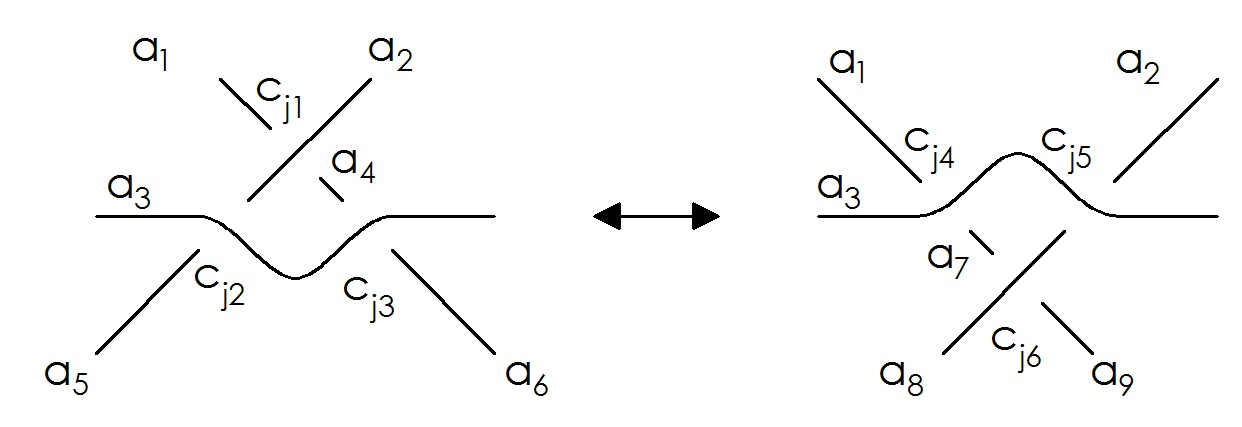
\includegraphics[scale=0.2]{2/Obrazy/R3}
		\end{center}
	\end{minipage}
	
\end{enumerate}
\end{proof}

\begin{lemat}
Jeżeli dla diagramu L istnieje kolorowanie $\lbrace a_{1}, \ldots , a_{k} \rbrace$, to dla każdego l $\in \N\:\: \lbrace a_{1}+l, \ldots , a_{k}+l \rbrace$ też jest kolorowaniem.
\end{lemat}
\begin{proof}
Dla każdego $c_{j}$ spełnione jest:\\
$a_{m11}+a_{m2}-2a_{m3} \equiv 0$ mod n. Wobec czego \\ 
$a_{m1}+l+a_{m2}+l-2a_{m3}-2l \equiv 0$.
\end{proof}
\textbf{Wniosek:} Jeśli diagram jest kolorowalny to istnieje kolorowanie takie że $a_{1} = 0$.

\paragraph{Kolorowanie modulo 2} Jeżeli węzeł jest kolorowalny modulo 2 to dla każdego skrzyżowania zachodzi jedna z czterech możliwości:
	\begin{center}
			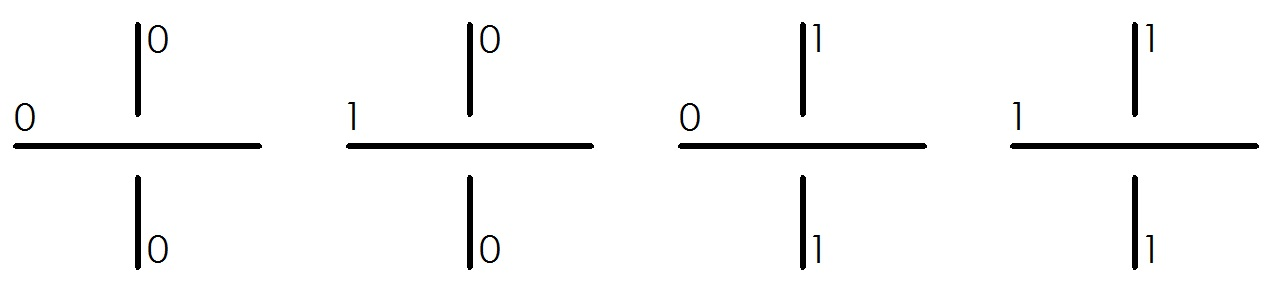
\includegraphics[scale=0.3]{2/Obrazy/Mod2}
	\end{center}
	W każdym przypadku kolory łuków leżących po przeciwnych stronach skrzyżowania są jednakowe. Startując w dowolnym punkcie węzłą i przechodząc go w wybranym kierunku otrzymamy że każdy łuk należący do tej samej komponenty spójności co punkt startowy ma przyporządkowany jednakowy kolor. Zatem węzeł może być kolorowany mod 2 $\Leftrightarrow$ węzeł ma więcej niż jedną komponentę spójności.
	
	\begin{definicja}
	Węzeł K jest podzielny jeśli ma conajmniej 2 komponenty spójności, oraz  $\exists U, V\:  otwarte, U \cap V = \emptyset$, takie że $ K\subseteq U\cup V, K\cap U \neq \emptyset, K\cap V \neq \emptyset$.
	\end{definicja}
	
	
\begin{lemat}
	Jeżeli węzeł K jest podzielny to, $\forall n >1 \:\:$ diagram L jest kolorowalny mod n.
\end{lemat}
	
\begin{proof}
Niech każdy łuk zawarty w U będzie pokolorowany na kolor 0, łuk zawarty w V na kolor 1. Takie przyporządkowanie jest kolorowaniem. Równania skrzyżowań zachodzą dla każdego n. 
\end{proof}

	
\subsection{Równania kolorowań}
\begin{definicja}
Krótki łuk, to część łuku który przechodzi dokładnie przez 2 skrzyżowania. 
\end{definicja}
\begin{definicja}
Region to komponenta spójności $\R^{2} \setminus L$.
\end{definicja}
\begin{definicja}
Szachownica diagramu to przyporządkowanie każdemu regionowi jednego z 2 kolorów tak aby każdy krótki łuk oddzielał regiony o różnych kolorach.
\end{definicja}

\textbf{Przykład:} Węzeł $7_{3}$ posiada 7 łuków, 14 krótkich łuków, 9 regionów.

			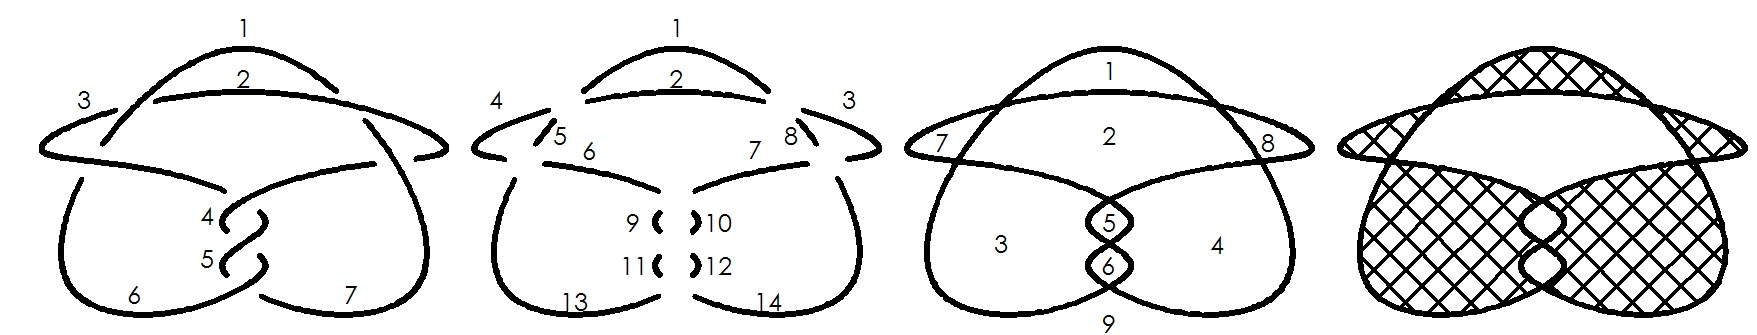
\includegraphics[scale=0.3]{2/Obrazy/ArcRegion3} \\


Dla każdego skrzyżowania $c_{j}$ równanie można przedstawić na 2 sposoby. 
\begin{definicja}
Wybór znaku równania nazywa się dobrym, gdy zachodzi następujący warunek. 
\end{definicja}

	\begin{minipage}{0.5\textwidth}
$a_{m2}+a_{m3}-2a_{m1} \equiv 0$ mod n, dla \\	
	\begin{center}
			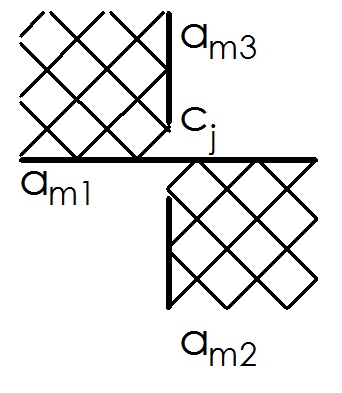
\includegraphics[scale=0.3]{2/Obrazy/Cros+}
	\end{center}
	\end{minipage}
	\begin{minipage}{0.5\textwidth}
$2a_{m1}-a_{m2}-a_{m3} \equiv 0$ mod n, dla \\
	\begin{center}
			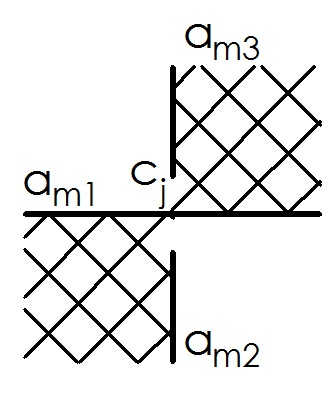
\includegraphics[scale=0.3]{2/Obrazy/Cros-}
	\end{center}	
	\end{minipage}

\begin{twierdzenie}
Suma równań po wszystkich skrzyżowaniach równa się 0, o ile znaki równań zostały \emph{wybrane dobrze}.
\end{twierdzenie}
\begin{proof}
Ustalmy dowolny krótki łuk $a_{j}$. $a_{j}$ pojawia się dokładnie w 2 równaniach skrzyżowań. Łuk łączy 2 skrzyżowania $c_{j1}$ oraz $c_{j2}$. Istnieje region $X_{1}$, taki że oba skrzyżowania graniczą z $X_{1}$. Bez straty ogólności $X_{1}$ jest białe. 
\begin{center}
  			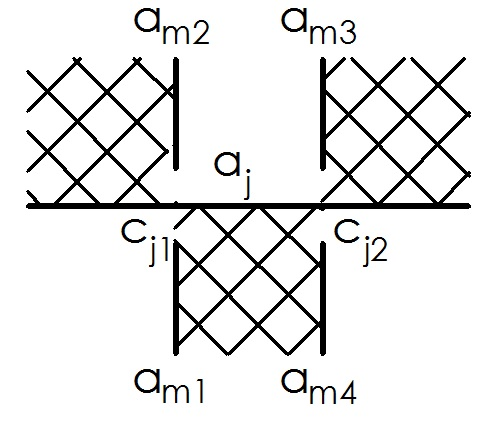
\includegraphics[scale=0.3]{2/Obrazy/0sum}
\end{center}
Ponieważ znaki równań zostały  \emph{wybrane dobrze}, znak $a_{j}$ w równaniu skrzyżowania  
$c_{j1}$, jest przeciwny do znaku $a_{j}$ w równaniu skrzyżowania $c_{j1}$. Wobec czego równania sumują się do 0.
\end{proof}


\subsection{Macierze kolorowań}
\subsection{Grupy kolorowań}
